\section{Computational model describing the PMT response}

The goal for using MAPMTs in RICH detectors is to achieve reliable detection of single photons in the Cherenkov light radiation cones. A single photon incident on a PMT face may knock out a single photoelectron from the PMT's photocathode with a certain probability, defined as Quantum Efficiency (QE). The photoelectrons cascade inside the PMT to generate a typical amplified electrical signal at the anode. The amplitude distribution of the single photoelectron (SPE) signal depends on the MAPMT design and high voltage applied, and varies from pixel to pixel. Tests and characterization of multiple MAPMTs include measuring the SPE amplitude distributions for every pixel, finding out the appropriate amplitude thresholds, and determining QE. To achieve this goal we used the methods developed in Ref.~\cite{DEGTIARENKO20171}, expanded to include the new empirical method to take into account the effects of the pixel-to-pixel crosstalk in H12700 tubes. The reference~\cite{DEGTIARENKO20171} describes in detail the computational model used to extract and parameterize the SPE distributions from the measurements using the laser test setup. The method allows in principle to describe the SPE functions of essentially any complexity by decomposing them into a sum of Poisson distributions with different averages. For the detailed explanations and the definition of the model parameters please refer to~\cite{DEGTIARENKO20171}. The list of main parameters includes $\mu$, average number of photoelectrons produced by the laser in a given pixel per one test pulse, and {\it{scale}}, average amplitude of the SPE distribution in pC. 
The parameter {\it{scale}} is directly connected with the $gain$ (or {\it{current amplification}}) parameter usually given in the photomultiplier specifications. The term $scale$ was introduced in Ref.~\cite{DEGTIARENKO20171} to handle the spectral data not necessarily normalized to the unit charge, and it is kept for compatibility. The value of $scale$ equal to 160.2~pC corresponds to $gain=10^6$, and the value of $gain$ may be obtained by multiplying $scale$ (in pC) by 6241.5.
Five model parameters determine the shape of the SPE distribution, defined as a normalized sum of three Poisson distributions with different average multiplication coefficients  applied to the photoelectron on the first dynode of the PMT. Average multiplication on the first cascade ${\nu}$, or ${\nu_{average}}$ (equivalent to the {\it secondary emission ratio} as per Hamamatsu PMT Handbook~\cite{Hamamatsu4thedition}) may be derived from these parameters. 
Parameter ${\sigma}$ describes the Gaussian shape of the pedestal function. ${\xi}$ parameter describes effective cascade multiplication on the second dynode. The combination of 9 parameters describes a single-anode PMT SPE response in an ideal measurement setup with a Gaussian pedestal function. If the pedestal amplitude distribution is not exactly following the Gaussian shape the problem of parameterizing the SPE distribution requires addition of new parameters taking into account the distortion of the pedestal Gaussian. The method was successfully implemented in~\cite{DEGTIARENKO20171} in the case of small exponential noise contribution to the Gaussian measurement function. In the present work we use similar ad hoc approach to parameterize and approximate the contribution of the crosstalk signals coming from the neighboring pixels to the SPE amplitude distribution. The model for the process, in agreement with the observations presented in the previous chapter, assumes that a portion of the signal from a neighboring pixel may be randomly added to the amplitude measured in a given pixel under investigation. Such random contribution could in principle depend on the neighbor. It would be very difficult to characterize all possible pair combinations separately. In the case of H12700 MAPMTs the signal amplitudes of the crosstalk contributions from different neighboring pixels were found to be relatively small and similar to each other, allowing us to use the single averaged spectral term for all neighbors of a given pixel. In the model every crosstalk contribution comes from a single electron in one of the neighboring pixels, their average number in one measurement $\beta$ is expected to be comparable with $\mu$, and multiple crosstalk events in one measurement happen independently. Average crosstalk contribution to the measurement function from one crosstalk electron corresponds to the second new model parameter $\zeta$, and the third new parameter $\lambda$ is introduced to adjust the shape of the crosstalk contribution. The explanation of the new formalism is given in Appendix A. It requires familiarity with the formulation of the model presented in full detail in Ref.~\cite{DEGTIARENKO20171}.

\begin{figure}[hbt]
	\centering
	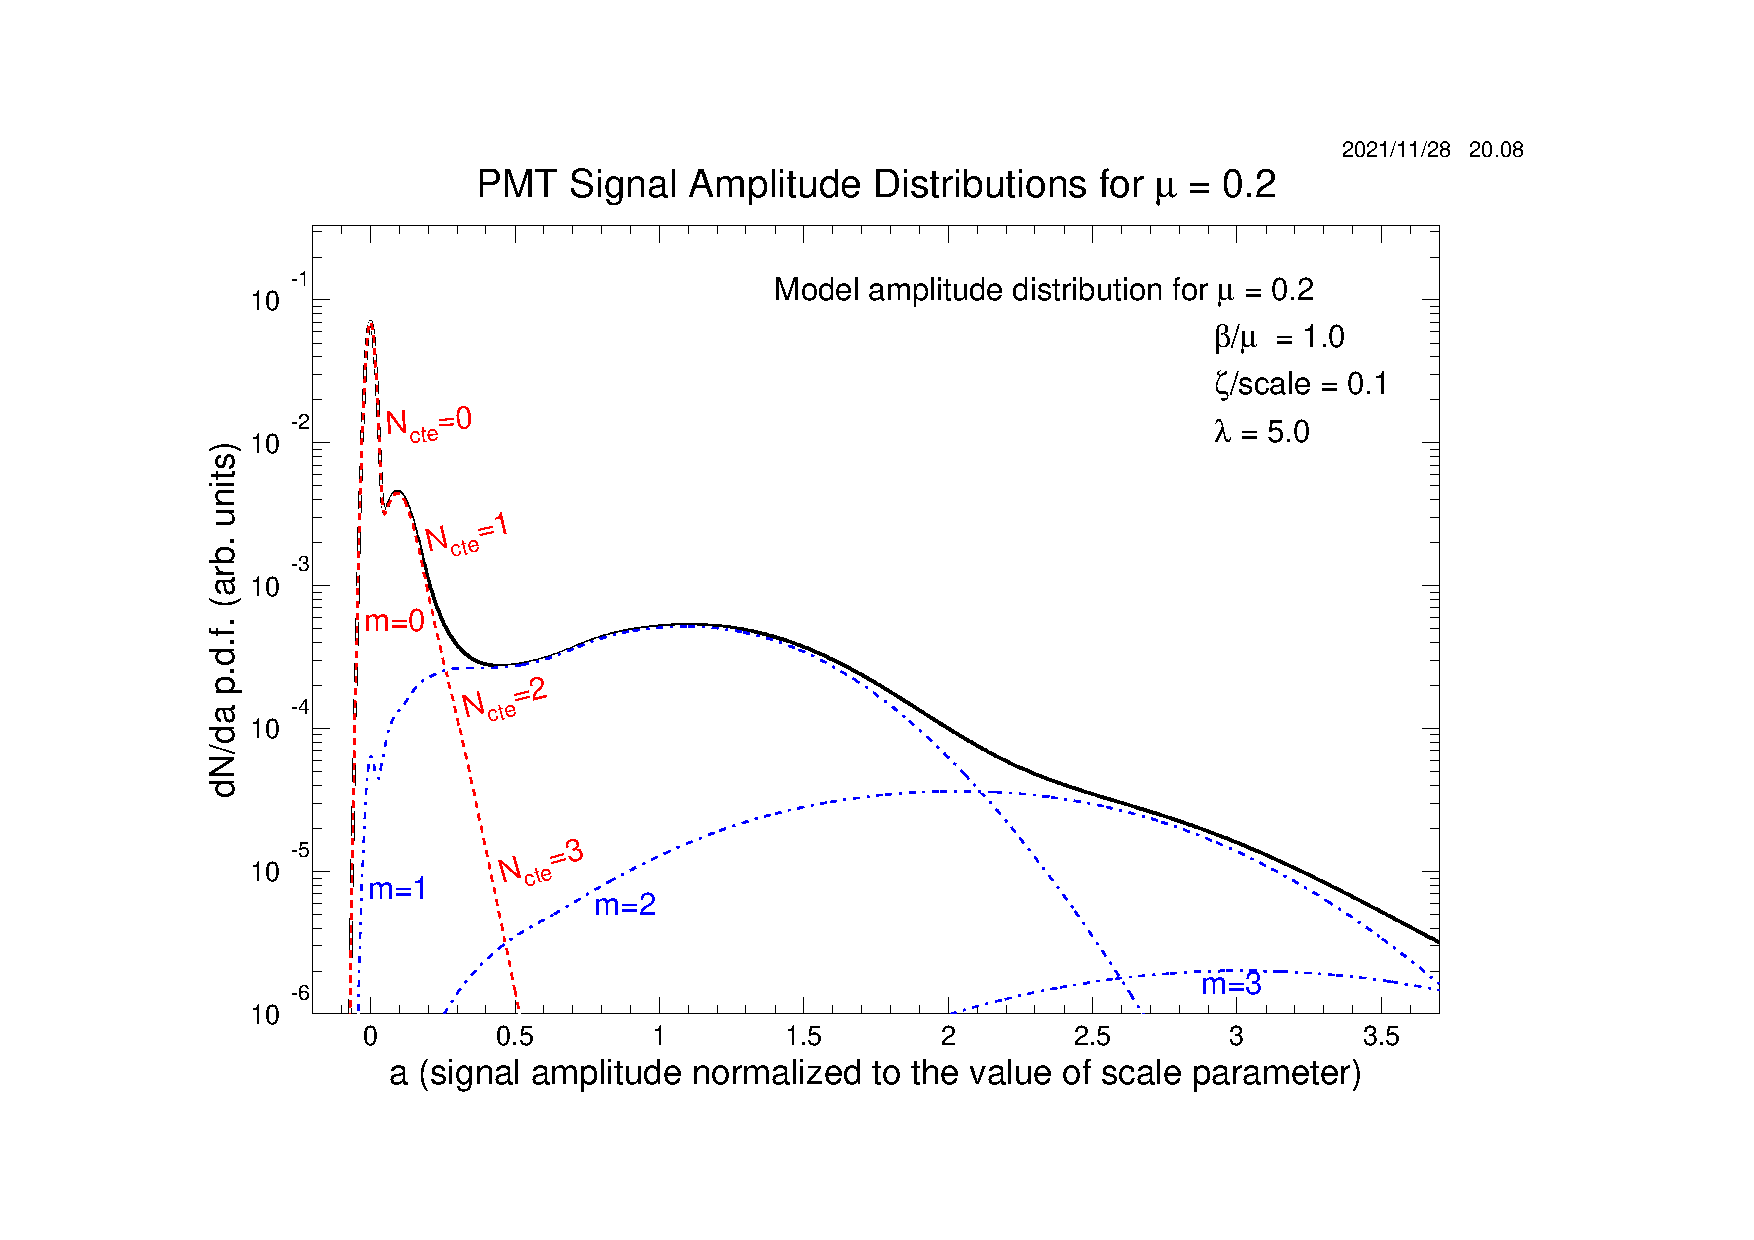
\includegraphics[width=0.98\linewidth, trim=80 55 105 105, clip]{figures/model.pdf}
	\caption{Model  signal  charge  distribution  (black  line)  illustrating  the parameterization for the crosstalk effects.  Red trace ($m=0$) corresponds to the pedestal measurement function with the additional crosstalk contribution, violet lines ($m$ = 1, 2, 3) show contributions from events with the number of photoelectrons 1, 2, and 3, with their relative probability corresponding to the Poisson distribution with average $\mu=0.2$}
	\label{fig:Model}
\end{figure}


The technique is illustrated in Fig.~\ref{fig:Model} showing an example of the distribution of the test events on the normalized measured charge $a$, with $a=1$ corresponding to the average charge collected from one photoelectron. The series of lines marked as $m = 1, 2, 3$ correspond to the charge distributions in the events with corresponding number of photoelectrons, assuming the average number of photoelectrons in test events is $\mu = 0.2$. Red distribution corresponds to the pedestal measurement function $R_{ct}(a)$ with the added crosstalk correction. Regions in this distribution marked with $\mathrm{N_{cte}=0, 1, 2, 3}$ correspond to the original Gaussian pedestal function and the contributions from one, two, and three crosstalk electrons. The parameters are selected for better visibility of the crosstalk effects, with $\beta$ equal to $\mu$, $\zeta$ equal to 10\% of the $scale$ parameter, and $\lambda = 5$ to make the crosstalk Poisson peak more visible.  

The fitting procedure from Ref.~\cite{DEGTIARENKO20171} was modified to include the new three parameters in the FORTRAN routine describing the measured test spectra, bringing the total number of parameters to 12. The algorithm for the multiparametric minimization was adjusted correspondingly to provide stability. The experimental verification of the fit stability and reproduceability of the results was performed using multiple measurements of the same MAPMTs in the different slots in the test setup and comparing the results. Overall confidence was assured by extracting parameters for each MAPMT in several test conditions, varying the high voltage and the illumination conditions, and verifying the consistency in the values of the extracted parameters. The procedure also helped us to evaluate the uncertainties of the major extracted model parameters.
